In this section, the derivation of the plant transfer function will be investigated. To start with, we focused on the mechanical part of the system and obtained the transfer function between $X$ and $\theta$. Our calculations can be seen from Figure \ref{fig:mechanical_transfer} below. \\

\begin{figure}[H]
    \centering
    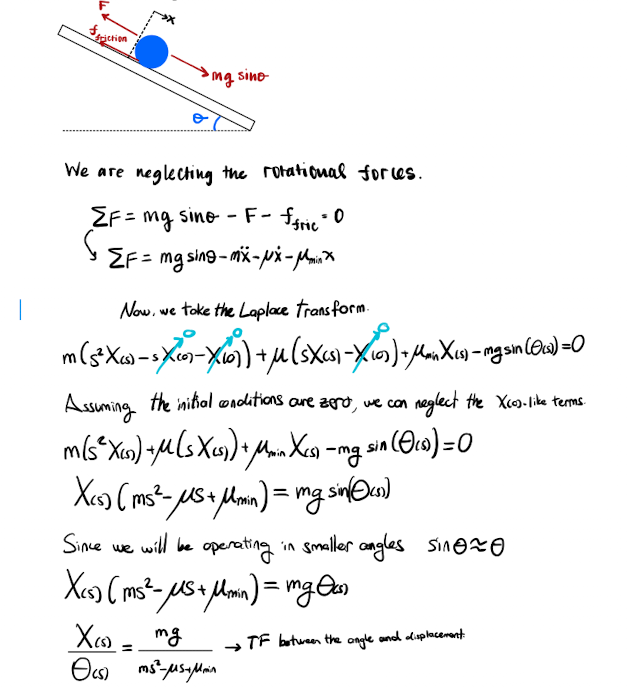
\includegraphics[width=.9\textwidth]{images/mechanical_transfer.png}
    \caption{Calculations of the first part}
    \label{fig:mechanical_transfer}
\end{figure}

\newpage

Following these calculations, $\theta$ will be related to our current, $I$. After this step, two equations can be combined easily to obtain the transfer function between the current and $X$. Figure \ref{fig:final_transfer} shows the steps and derivations for these equations. 

\begin{figure}[H]
    \centering
    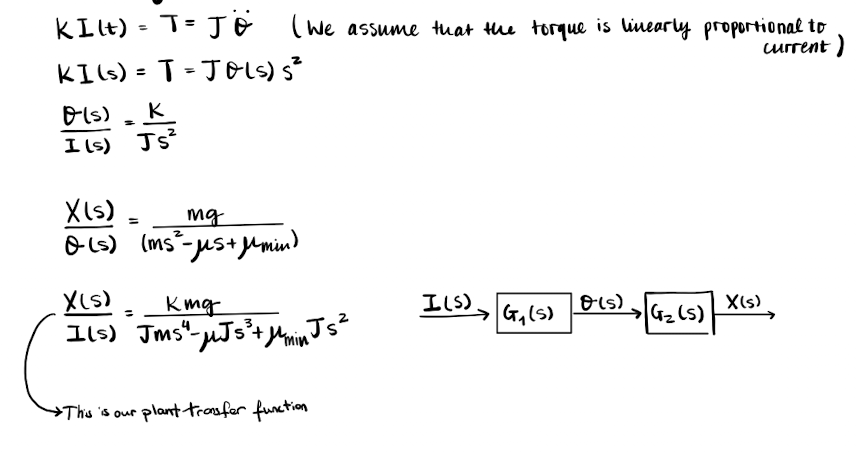
\includegraphics[width=.9\textwidth]{images/second_transfer.png}
    \caption{Derivation of the transfer function}
    \label{fig:final_transfer}
\end{figure}

Our transfer function is shown at the end of Figure \ref{fig:final_transfer}. Plugging in the values from the project prompt, our transfer function becomes as follows:

\begin{equation}
    T(s) = \frac{ 0.0981}{s^4 + 5 s^3 + 20 s^2}
\end{equation}